\section{SITRA-exercise}
One of the first group exercises proposed by the facilitators was the SITRA-exercise. In this exercise we were handed a SITRA-sheet where different aspects where colour coded, and we were to evaluate the previous group reflection based on these colours. The colours helped evaluate the group reflections and give us an idea of where on the grading scale the reflections was, by giving different aspects, as shown in \autoref{fig:sitra}. 

During this exercise the group discovered that we had written our first group reflection chiefly by explaining a situation followed by a reflection, both of them quite short and uninformative. This led to a larger focus on a deeper group reflection, with more theory and action considerations where that was applicable. The group felt that the exercise helped give a more objective view on how to write the group reflections, based on how they would be graded.
\newpage{}
\begin{figure}
	\begin{center}
		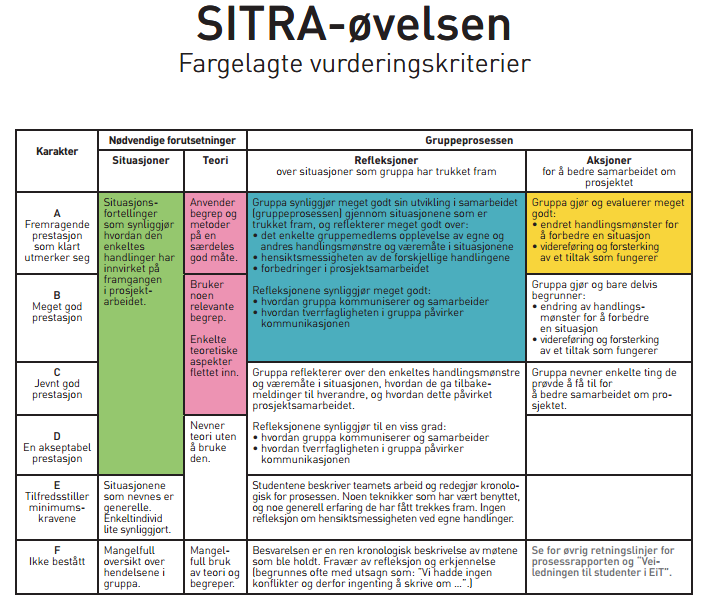
\includegraphics[width=0.7\textwidth]{Figures/sitra.png}
	\end{center}
	\caption[The SITRA Exercise]{The SITRA-sheet given for the SITRA exercise}
	\label{fig:sitra}
\end{figure}